\documentclass[aspectratio=169,t]{beamer}
\usepackage[utf8]{inputenc}
\usepackage[T1]{fontenc}


\title{Einführung in die Gesundheits\-informatik}
\date{WS 2019/2020}
\author[PWD]{Dr.-Ing. Piotr Wojciech Dabrowski}

\usepackage{HTWBeamerTemplate/beamerthemeHTW}
\addbibresource{Bilder/imagesources.bib}
\begin{document}

\setbeamertemplate{background}[bgfirst]
\setbeamertemplate{footline}[first]
\subtitle{0: Allgemeines}
\titlegraphic{Bilder/logo.png}
\begin{frame}[noframenumbering]
\titlepage
\end{frame}
\setbeamertemplate{footline}[presentationbody] 
\setbeamertemplate{background}[bgbody]

\begin{frame}{Vorstellung}
 \begin{itemize}
     \item<2-> Kurz zu mir
     \only<2-5>{
      \begin{itemize}
        \note<2>{Um zu verstehen, was ich weiß und was ich nicht weiß}
        \item<2-5> Kontakt: Piotr.Dabrowski@posteo.de - gerne nutzen!
        \item<3-5> Geboren 1981 in Warschau
        \item<3-5> Studium der Biotechnologie \& Informatik an der TU Berlin
        \item<3-5> Promotion über Auswertung von Hochdurchsatzdaten für Virus-Diagnostik
        \item<3-5> Aufbau der bioinformatischen Analytik für das NGS-Labor des RKI
        \item<3-5> Aufbau der Bioinformatics Core Facility am RKI
        \note<3>{Entsprechend andere Schwerpunkte der VL, als bisher\\Gesundheitsinformatik ist nicht gleich Bioinformatik!}
        \item<4-5> Seit WS 2019/2020 an der HTW
        \note<4>{Erste Vorlesungen an der HTW:
            \begin{itemize}
                \item Lerne erst Modalitäten kennen
                \item Kenne die Vorkenntnisse/präferierte Art der Studierenden nicht
                \item Primäres Ziel: Verständnis aufbauen, "durch den Stoff kommen" zweitrangig
                \item Also bitte (rechtzeitig) melden, wenn Interesse an Vertiefung besteht
                \item Gemeinsame Reise - bitte immer melden, wenn was ist!
                \item Gerne auch außerhalb der Sprechzeiten, wenn die Tür offen ist einfach reinkommen.
            \end{itemize}
        }
        \item<5> Hang zum Experimentieren in der Vorlesung - Feedback erwünscht!
        \note<5>{
        \begin{itemize}
            \item Gruppenarbeiten
            \item Mini-Whiteboards
            \item Angebot: Treppenlauf
            \item Bitte melden, wenn es zu viel wird!
        \end{itemize}}
      \end{itemize}
     }
     \item<6-> Der Todesstern \& (ausgewählte) andere Hilfsmittel
     \item<10-> Sie \& Ihre Vorstellungen von der Gesundheitsinformatik
     \note<10>{
     Ziele:
     \begin{itemize}
         \item Kennenlernen der Vorkenntnisse und Wünsche
         \item Eventuell Anpassung der Schwerpunkte später im Semester
         \item Eigene Auseinandersetzung hilft beim Erinnern
         \item Aber erst mal Allgemeines fertig, dann dieser Teil der Vorstellung!
     \end{itemize}
     }
 \end{itemize}
 \only<6-9>{
  \begin{textblock}{15}(2,7)
   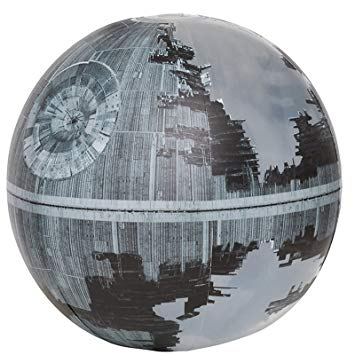
\includegraphics[width=3cm]{Bilder/Todesstern.jpg}
  \end{textblock}
 }
 \only<7-9>{
  \begin{textblock}{15}(5.5,8.25)
   
\includegraphics[width=3cm]{Bilder/Tischnamensschild.png}
  \end{textblock}
 }
 \only<8-9>{
  \begin{textblock}{15}(9,7.5)
   
\includegraphics[angle=77,origin=c,height=2cm]{Bilder/Tischnamensschild.png}
  \end{textblock}
 }
 \only<9>{
  \begin{textblock}{15}(11.5,8)
   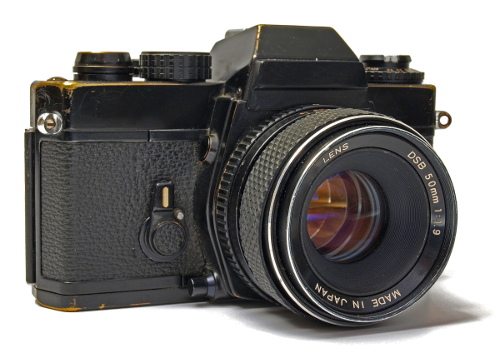
\includegraphics[width=3cm]{Bilder/DSLR.png}
  \end{textblock}
 }
\end{frame}

\begin{frame}{Inhalt der Vorlesung}
 Was macht Informatik im Gesundheitswesen? \uncover<2->{Am Beispiel eines Patienten mit Tuberkulose oder Krebs.}
\note<2>{
 \begin{itemize}
     \item Differentialdiagnostik z.T. interessant, werden wir gleich sehen.
     \item Generell drei Aspekte:
     \begin{itemize}
         \item Gesundheitswesen/Diagnostik/Einsatz im Krankenhaus
         \item Biologische Grundlagen
         \item Programmierung
     \end{itemize}
 \end{itemize}
}
 \begin{itemize}
     \item<3-> Gesundheitssystem allgemein
     \only<3>{\begin{itemize}
        \item Wo kommt das Geld für die Behandlung her?
        \item Wer regelt was wann wie gemacht wird?
        \item Welche Daten werden wo gespeichert? 
     \end{itemize}}
     \item<4-> Molekulare Diagnostik
     \only<4>{\begin{itemize}
        \item Erregernachweise (ELISA, PCR)
        \item Grundlagen der Arbeit mit Bilddaten
     \end{itemize}}     
     \item<5-> Bildgebende Verfahren
     \only<5>{\begin{itemize}
        \item Blick in das Gewebe: Ultraschall, Röntgen, \\CT, MRT, OCT
        \item Ein wenig Mathematik (Fourier-Transformation)
        \item Fortgeschrittenere Bilddatenverarbeitung
     \end{itemize}}     
     \item<6-> DNA-basierte Hochdurchsatz-Diagnostik
     \only<6>{\begin{itemize}
        \item Microarrays, Next Generation Sequencing
        \item Einige Methoden des maschinellen Lernens
        \item Krebsdiagnostik
     \end{itemize}}     
     \item<7-> Proteomik
     \only<7>{\begin{itemize}
        \item Tandem-MS
        \item Wie sicher ist man sich, es falsch \\gemacht zu haben?
        \item Verbesserte Krebsdiagnostik
     \end{itemize}}     
 \end{itemize}
 \only<3>{
  \begin{textblock}{10}(7.5,4.5)
   \begin{figure}[h!]
     \label{figure:VDEK}
     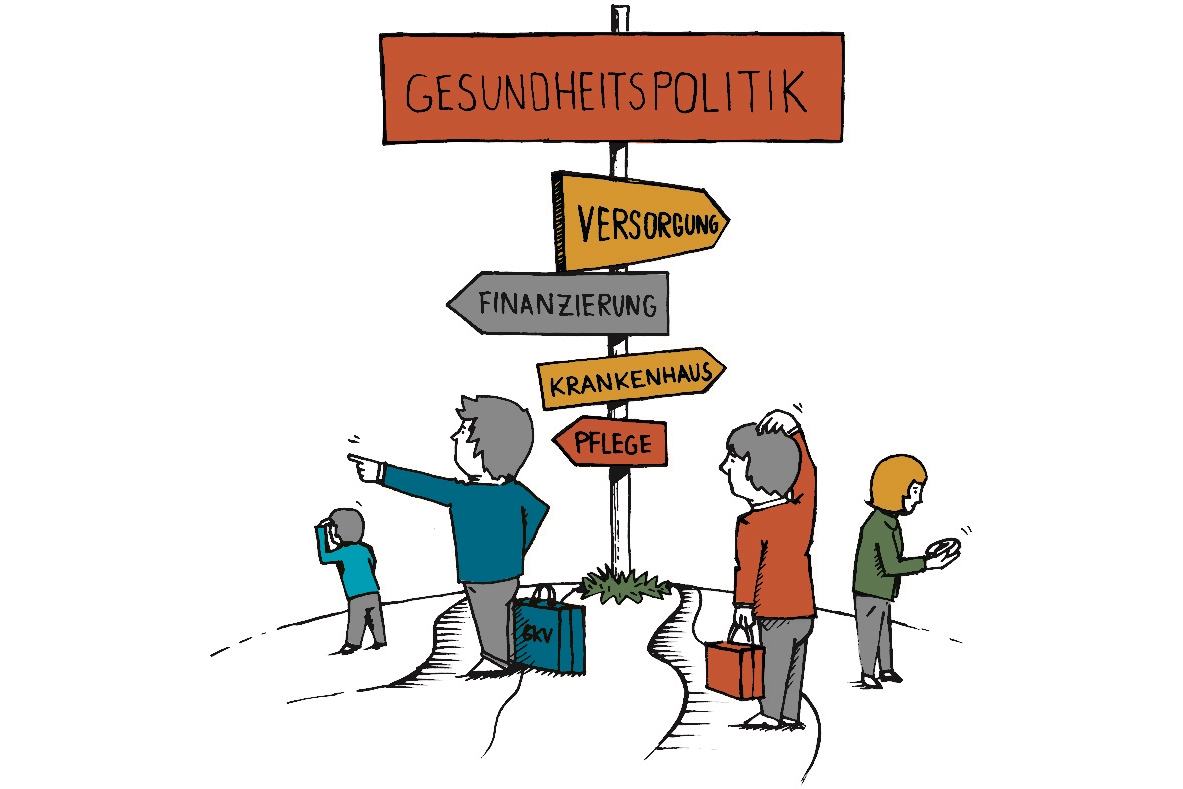
\includegraphics[width=7.5cm]{Bilder/Gesundheitspolitik.png}
     \caption{Cartoon von VDEK \cite{VDEK}}
   \end{figure}
  \end{textblock}
 }
 \addtocounter{figure}{1}
 \only<4>{
  \begin{textblock}{10}(7,4.5)
   \begin{figure}[h!]
     \label{figure:ELISA}
     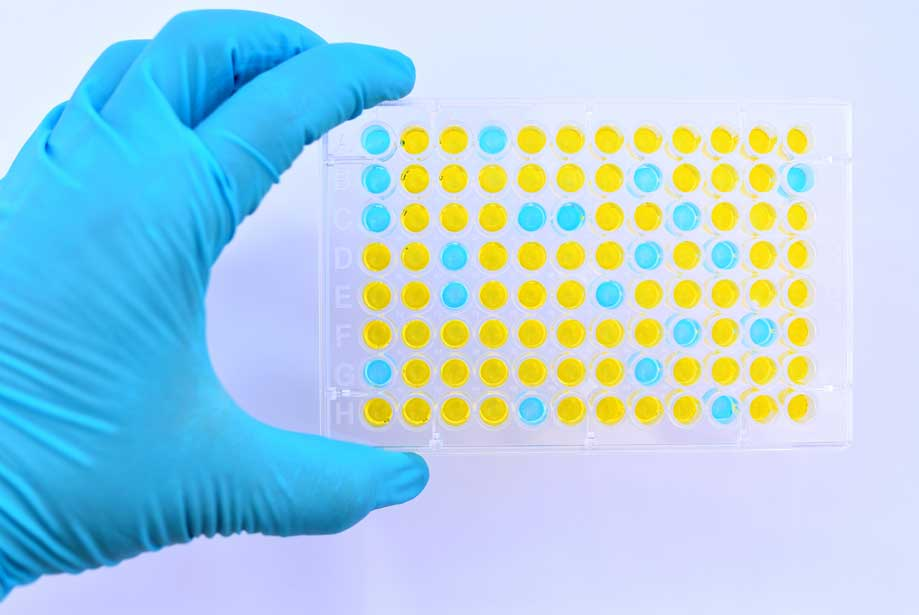
\includegraphics[width=7.5cm]{Bilder/ELISA.jpg}
     \caption{ELISA-Platte \cite{ELISA}}
   \end{figure}
  \end{textblock}
 }
 \addtocounter{figure}{1}
 \only<5>{
  \begin{textblock}{10}(7.5,4.5)
   \begin{figure}[h!]
     \label{figure:CT}
     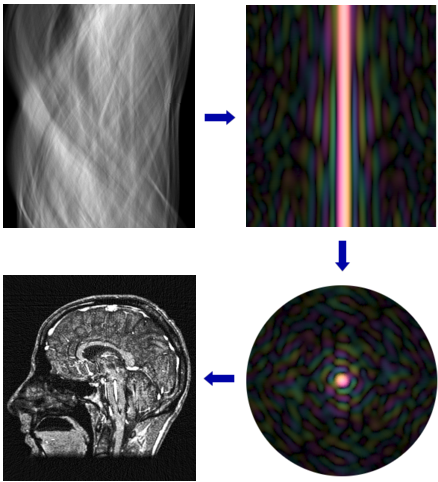
\includegraphics[width=4.5cm]{Bilder/CT.png}
     \caption{Radon-Transformation \cite{Radon}}
   \end{figure}
  \end{textblock}
 }
 \addtocounter{figure}{1}
 \only<6>{
  \begin{textblock}{10}(7.5,4.5)
   \begin{figure}[h!]
     \label{figure:NGS}
     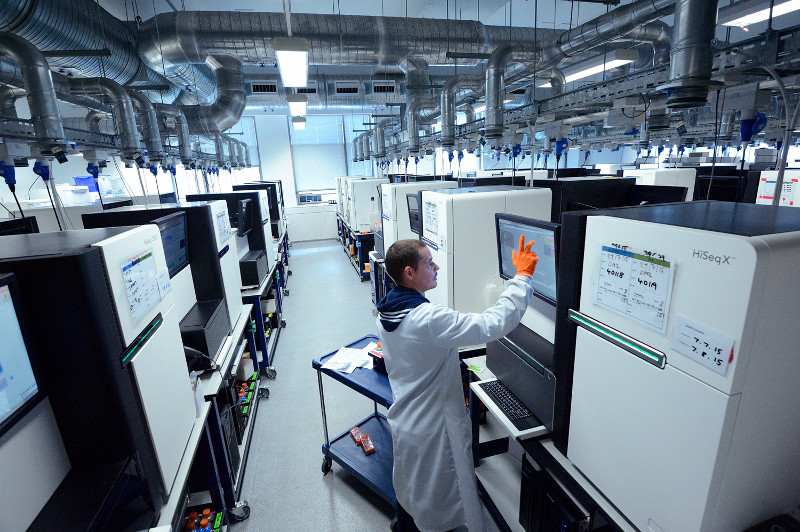
\includegraphics[width=6.5cm]{Bilder/NGS.jpg}
     \caption{NGS-Labor am Sanger Institute \cite{NGS}}
   \end{figure}
  \end{textblock}
 }
 \addtocounter{figure}{1}
 \only<7>{
  \begin{textblock}{10}(7,4.5)
   \begin{figure}[h!]
     \label{figure:HPLCMS}
     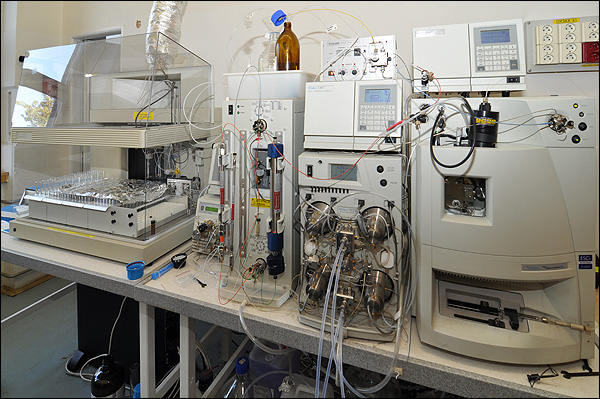
\includegraphics[width=6.5cm]{Bilder/LCMS.jpg}
     \caption{Ein (älteres) Massenspektrometer \cite{LCMS}}
   \end{figure}
  \end{textblock}
 }
\end{frame}

\begin{frame}{Inhalt der Übung}
 \begin{itemize}
     \item Firmenbesuche
     \only<2>{
      \begin{itemize}
        \item VmScope GmbH
        \item Berlin Heart GmbH
        \item MicroDiscovery GmbH
        \item RKI (NGS-Lab, Proteomik \& Bioinformatik)
      \end{itemize}
     }
     \note<2>{
       Zur Steigerung der Aufmerksamkeit: Kurztestate nach Besuch der Firmen, 2-3 Fragen zur Firma auf max. 1/2 A4-Seite zu beantworten.
     }
     \item Softwareentwicklung basierend auf Vorlesungs-Inhalten
     \item Kurzvorstellungen der Übungsergebnisse
 \end{itemize}
\end{frame}

\begin{frame}{Gesamtfahrplan (vorläufig)}
  \note{Vorläufig, je nach:
   \begin{itemize}
       \item Allgemeinem Vorankommen (gründlich verstehen wichtiger als kompletten Stoff durchprügeln)
       \item Terminverschiebungen bei Firmen
   \end{itemize}
  }
  \begin{columns}
   \begin{column}{0.5\textwidth}
  \begin{itemize}
    \item KW41: Gesundheitssystem
    \item KW42: Molekulare Diagnostik % und Grundlagen Python
    \item KW43: Ü: Datenauswertung in Python
    \item KW44: Ü: Datenauswertung in Python
    \item KW45: Besuch: Berlin Heart
    \item KW46: Bildgebende Verfahren
    \item KW47: Besuch: VmScope
    \item KW48: Ü: Bilddatenauswertung
  \end{itemize}
   \end{column}
   \begin{column}{0.5\textwidth}
  \begin{itemize}
    \item KW50: Besuch: MicroDiscovery
    \item KW51: Ü: Microarray-Auswertung
    \item KW02: NGS
    \item KW03: Besuch: RKI
    \item KW04: Ü: NGS-Auswertung
    \item KW05: Ergebnisvorstellung
%    \item KW50: 
%    \item KW50: 
%    \item KW44: Python-Grundlagen, Auswertung von Daten aus molekularer Diagnostik
%    \item KW46: Fortgeschrittenere Bilddaten-Auswertung
%    \item KW48: Besuch der MicroDiscovery GmbH (Auftragsdatenauswertung, Microarrays)
%    \item KW50: Auswertung von Microarray-Daten
%    \item KW02: Besuch des RKI (NGS-Lab, Proteomik \& Bioinformatik)
%    \item KW04: Auswertung von NGS- und Proteom-Daten
  \end{itemize}
   \end{column}
  \end{columns}
   
\end{frame}

\begin{frame}{Benotung}
 \note<2>{Muss nicht ``fertig werden'', Idee und Herangehensweise ausschlaggebend.}
 \begin{itemize}
     \item<1-> Klausur: $30\%$
     \item<1-> Übungsaufgaben: $30\%$
     \item<1-> Firmen-Testate: $20\%$
     \item<1-> Ergebnisvorstellung: $20\%$
     \item<2-> Konsequente Verwendung von git für Übungsaufgaben: $10\%$ Bonus
     \item<3-> Fachliche Fehler in der Vorlesung:
     \begin{itemize}
         \item $5\%$ Bonus pro Fehler 
         \item Kumulativ, maximal $15\%$ pro Semester
     \end{itemize} 
     \item<4-> Akzeptierte Verbesserungen an Vorlesung/Handout:
     \begin{itemize}
         \item $2.5\%$ Bonus pro Fehler, $5\%$ falls per pull request
         \item Kumulativ, maximal $7.5\%$ pro Semester, $15\%$ falls per pull request
     \end{itemize} 
 \end{itemize}
\end{frame}

\begin{frame}{Optionaler Exkurs: git}
    
\end{frame}

\begin{frame}{Exkurs: Warum Python?}
  \only<2->{Was sind typische Aufgabenbereiche für Bioinformatiker?\vspace{0.3cm}}
  \note<2>{
   Vorsicht:
   \begin{itemize}
       \item Das bezieht sich alles primär auf Bioinformatik
       \item Medizininformatik: 99\% Windows
   \end{itemize}
  }
  \begin{columns}
   \begin{column}{0.5\textwidth}
     \only<3->{\centering \textbf{Softwareentwicklung}}
     \begin{itemize}
       \item<3->Produktzentriert
       \item<3->Performante Implementation eines Algorithmus
       \item<3->Stabilität, Reproduzierbarkeit, gutes User Interface
       \item<4->Primär Java, C++
     \end{itemize}
   \end{column}
   \begin{column}{0.5\textwidth}
     \only<5->{\centering \textbf{Datenauswertung}}
     \begin{itemize}
       \item<5->Projektzentriert
       \item<5->Verwendung existierender Tools
       \item<5->Entwicklung von Pipelines
       \item<5->Implementation kleinerer Algorithmen
       \item<5->Flexibilität, bedarfsgerechte Visualisierung
       \item<6->Primär Python, R
     \end{itemize}
   \end{column}
  \end{columns}
  \note<6>{
   Allgemein: Flexibilität ist wichtig!
   \begin{itemize}
       \item Java super für portable, performante Applikationen, aber mies für Prototyping
       \item Python super für Prototyping, aber schlecht für Stabilität
       \item PHP Totalausfall bei Wartbarkeit+Sicherheit, aber toll für schnelle kleine Webapp
       \item Wünsche JavaScript schnellen und schmerzhaften Tod, setze es trotzdem für interaktive Visualisierungen ein
   \end{itemize}
   Fazit: Keine silver bullet, man muss viele Stärken und Schwächen kennen, und z.T. Programmierkonzepte zwischen Sprachen übertragbar. 
  }
\end{frame}

\begin{frame}{Exkurs: Warum Python (II)?}
  \begin{textblock}{10}(1,2.8)
   \begin{figure}[h!]
     \frame{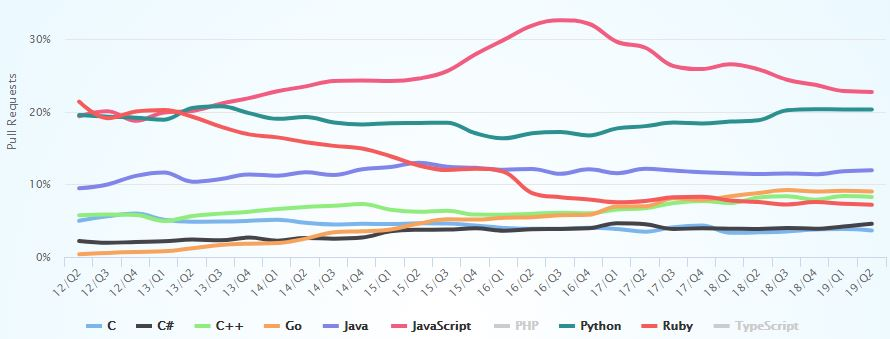
\includegraphics[width=12cm]{Bilder/PythonPulls.jpg}}
     \caption{Pull-requests auf github nach Sprache \cite{PythonPulls}}
   \end{figure}
  \end{textblock}
 \only<2->{
  \begin{textblock}{10}(0.9,3)
   \begin{figure}[h!]
     \frame{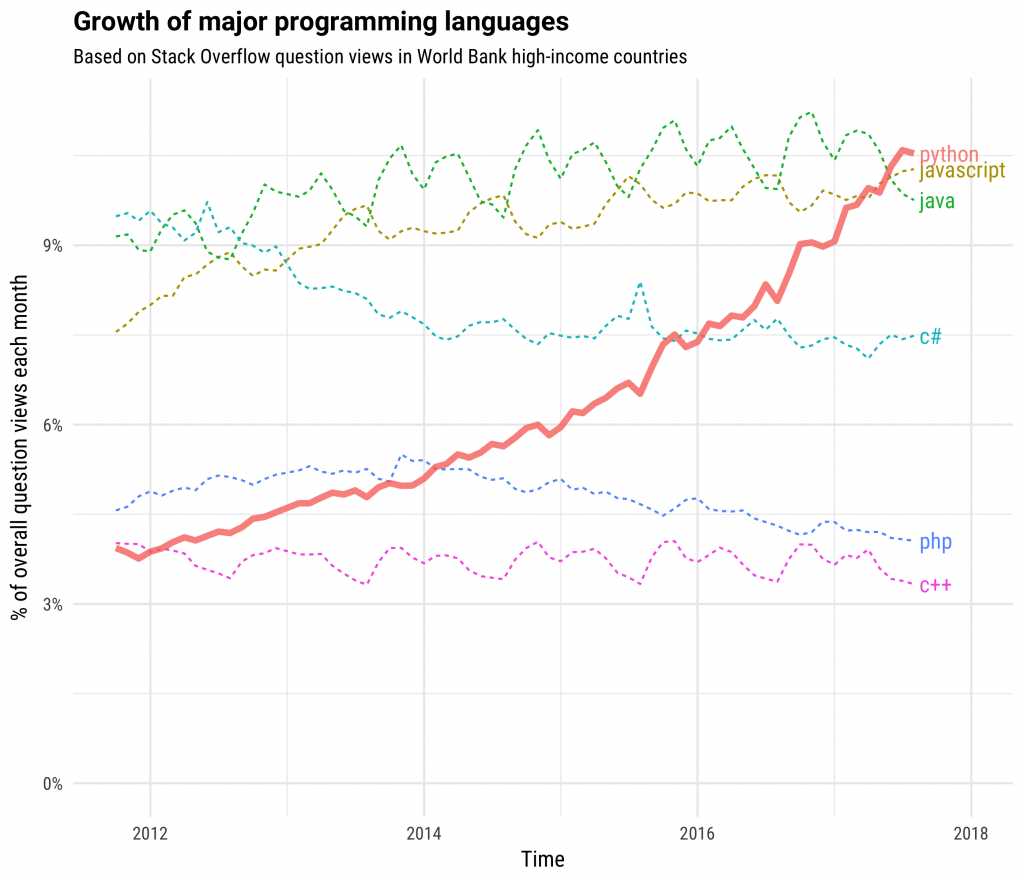
\includegraphics[width=6.5cm]{Bilder/PythonQuestions.png}}
     \caption{Fragen auf StackOverflow nach Sprache \cite{PythonQuestions}}
   \end{figure}
  \end{textblock}
 }
 \only<3->{
  \begin{textblock}{10}(7.1,0.6)
   \begin{figure}[h!]
     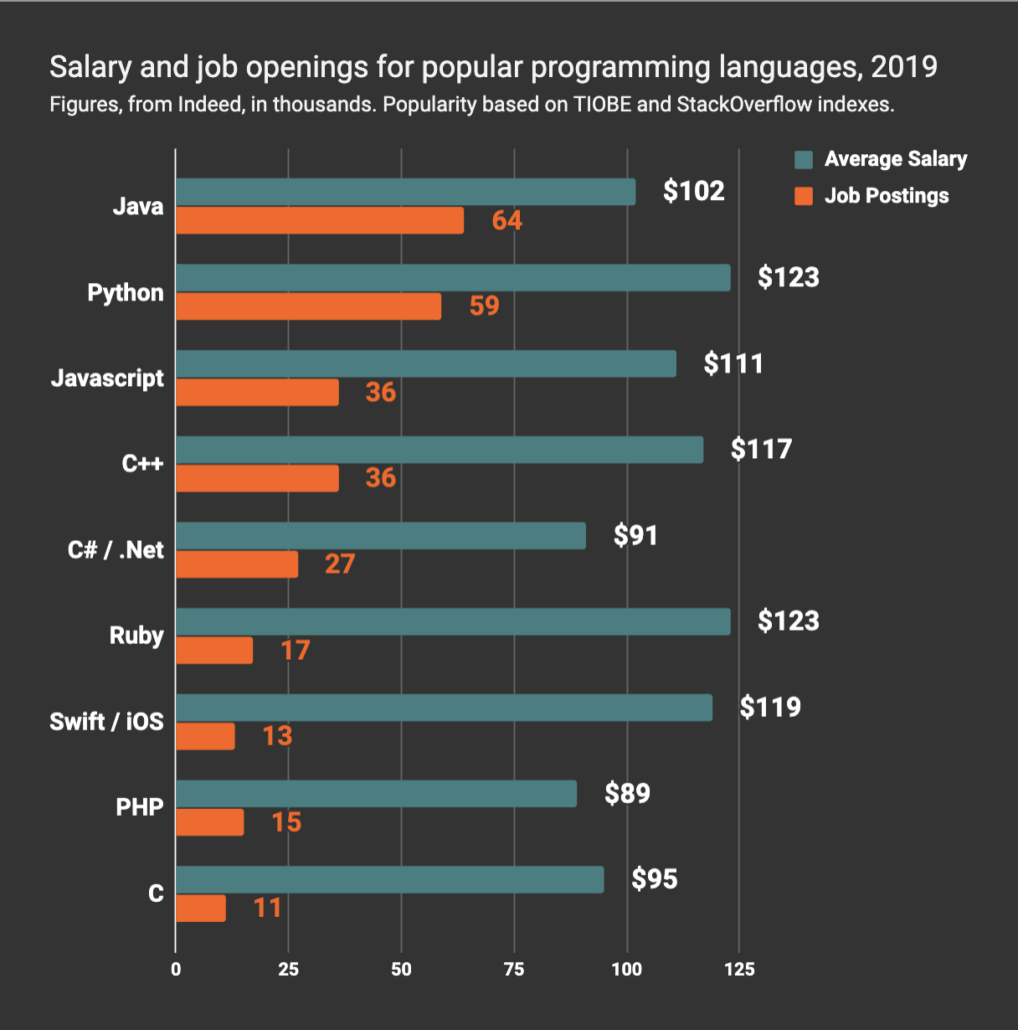
\includegraphics[width=7cm]{Bilder/LanguagesSalary.png}
     \caption{Einkommen und Stellen nach Programmiersprache \cite{LanguagesSalary}}
   \end{figure}
  \end{textblock}
 } 
\end{frame}


\setbeamertemplate{background}[bgfirst]
\setbeamertemplate{footline}[first]
\subtitle{1: Gesundheitssystem}
\titlegraphic{Bilder/logo1.png}
\begin{frame}[noframenumbering]
\titlepage
\begin{textblock}{10}(4.75,15)
\cite{GesundheitssystemLogo}
\end{textblock}
\end{frame}
\setbeamertemplate{footline}[presentationbody] 
\setbeamertemplate{background}[bgbody]

\begin{frame}{Begriffsdefinition(en)}
    \begin{definition}
        Das Gesundheitswesen ist die Gesamtheit eines organisierten Handelns als Antwort auf das Auftreten von Krankheit und Behinderung und zur Abwehr gesundheitlicher Gefahren.
    \end{definition}
    \only<2->{\begin{definition}
        Das Gesundheitswesen setzt sich aus allen Instituten, Einrichtungen, Personen und allen Maßnahmen zusammen, die für die Bevölkerung gesundheitsfördernd und -erhaltend sind, vorbeugend gegen Verletzungen und Krankheit wirken sowie diese behandeln.
    \end{definition}}
\end{frame}


\begin{frame}{Ihre Vorstellungen}
    \note{
         Gruppenarbeit:
      \begin{itemize}
          \item Informatik=Datenverarbeitung
          \item Gesundheitsinformatik=Datenverarbeitung im Gesundheitswesen
          \item Frage: Patient kommt mit Tuberkulose (Gruppe A) oder Krebs (Gruppe B) in's Krankenhaus. Welche Einrichtungen könnten beteiligt sein (direkt oder indirekt), wo werden Patientendaten verarbeitet (personenbezogen/anonym/statistisch)?
          \item Gruppengröße: 1 Reihe
          \item Zeit: 10 Minuten
      \end{itemize}
     }
     \only<2->{
       \begin{itemize}
           \item Tafelbild - coming to a git repo near you soon!
       \end{itemize}
    }
\end{frame}

\begin{frame}{Akteure im Gesundheitssystem (Überblick)}
   \begin{figure}[h!]
    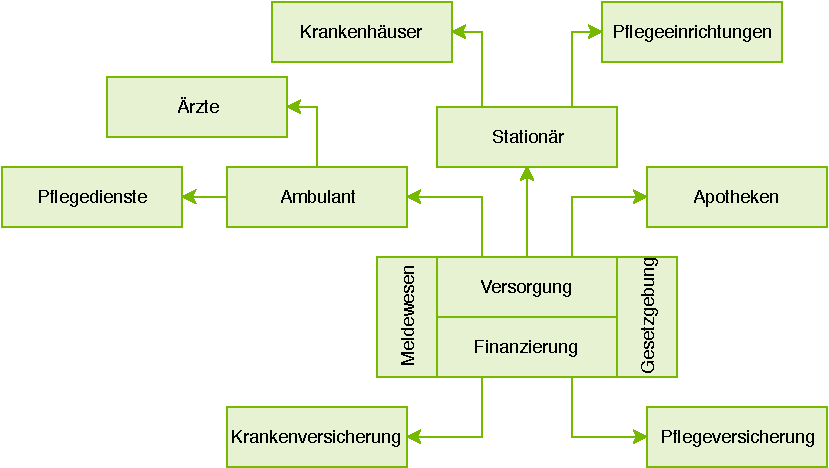
\includegraphics[height=5.5cm]{Bilder/Gesundheitssystem.pdf}
     \caption{Akteure im Gesundheitssystem. Eigene Abbildung in Anlehnung an \cite{SmartHealth}}
   \end{figure}
\end{frame}

\begin{frame}{...und ein kurzer Blick in die Tiefe}
   \begin{figure}[h!]
    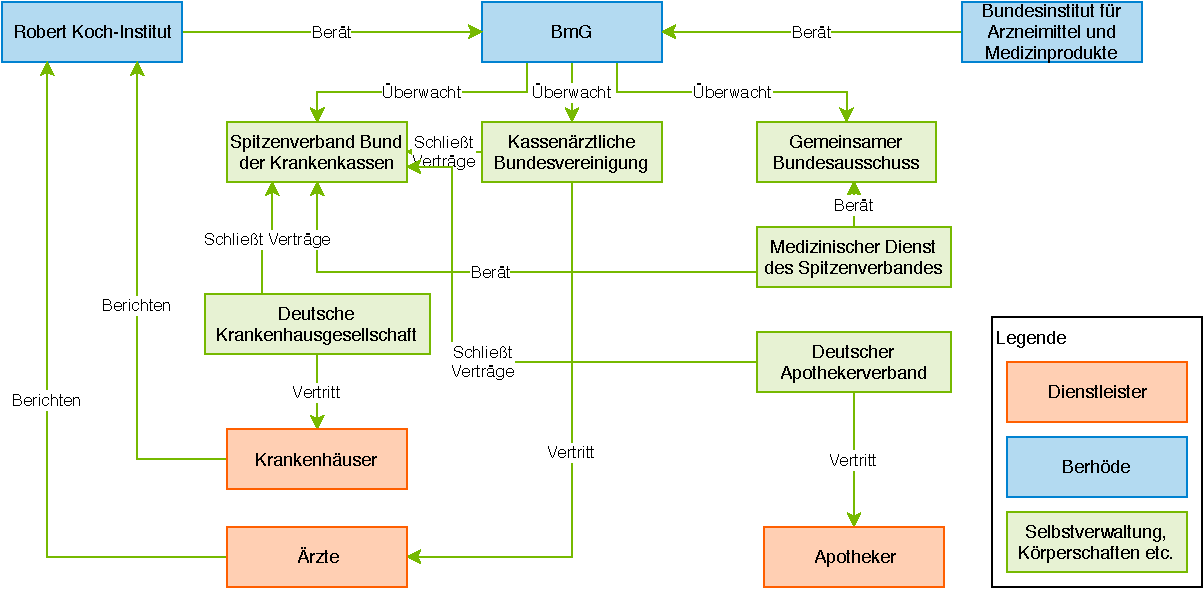
\includegraphics[height=5.5cm]{Bilder/GesundheitssystemAkteureBund.pdf}
     \caption{Einige Interaktionen auf Bundesebene. Eigene Abbildung.}
   \end{figure}
\end{frame}

\begin{frame}{...und ein kurzer Blick in die Tiefe}
   \begin{figure}[h!]
    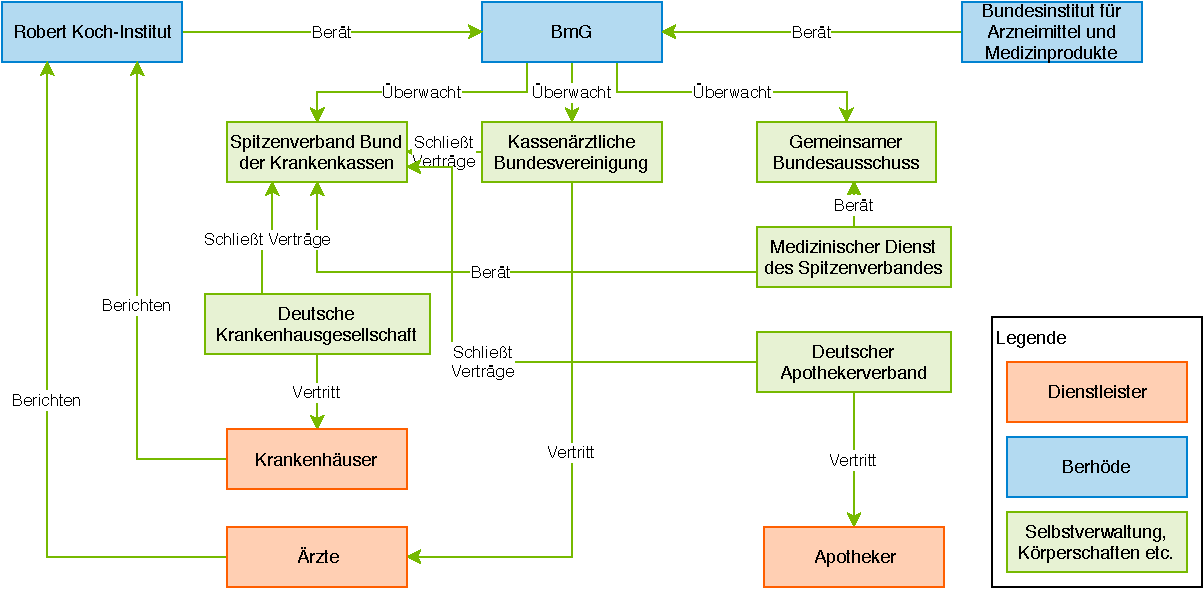
\includegraphics[height=5.5cm]{Bilder/GesundheitssystemAkteureBund.pdf}
     \caption{Einige Interaktionen auf Bundesebene. Eigene Abbildung.}
   \end{figure}
\end{frame}


\begin{frame}{Bildquellen}
\printbibliography
\end{frame}

\end{document}